\documentclass[10pt,a4paper]{article}
\usepackage[a4paper,margin=2.1cm,bottom=2.5cm,footskip=1.0cm]{geometry} % page number sits inside the border
\usepackage{fontspec}   % Tectonic = XeTeX: Unicode (±, –, ×, →) in generated tables
\usepackage{amsmath}
\usepackage{microtype}
\usepackage{graphicx}
\usepackage{booktabs}
\usepackage{tabularx}
\usepackage{array}
\usepackage{multirow}
\usepackage{xcolor}
\usepackage{listings}
\usepackage{caption}
\usepackage{subcaption}
\usepackage{enumitem}
\usepackage{float}
\usepackage{tikz}
\usetikzlibrary{positioning,fit,arrows.meta,backgrounds,calc,shapes.geometric}
\usepackage{eso-pic}
\usepackage{titlesec}
\usepackage[hidelinks]{hyperref}
\usepackage{cleveref}

% ---------------------------------------------------------------------------
% Cover-page details and group members — edit here only; they propagate through
% the cover page and the ownership table of the report.
% ---------------------------------------------------------------------------
\newcommand{\coursecode}{EC9110}
\newcommand{\coursename}{Modern Mobile Communication}
\newcommand{\assignmentname}{Assignment -- End-to-End 5G Simulation}
\newcommand{\semester}{Semester 07}
\newcommand{\submissiondate}{07 Oct 2026}

% Name and registration number of each member (component owned in the comment)
\newcommand{\nameA}{Member A}\newcommand{\idA}{2022/E/XXX} % Core network -- control plane
\newcommand{\nameB}{Member B}\newcommand{\idB}{2022/E/XXX} % Core network -- user plane
\newcommand{\nameC}{Member C}\newcommand{\idC}{2022/E/XXX} % Radio access network (gNB)
\newcommand{\nameD}{Member D}\newcommand{\idD}{2022/E/XXX} % UE and subscriber provisioning
\newcommand{\nameE}{Member E}\newcommand{\idE}{2022/E/XXX} % Traffic generation
\newcommand{\nameF}{Member F}\newcommand{\idF}{2022/E/XXX} % Signalling capture and analysis
\newcommand{\nameG}{Member G}\newcommand{\idG}{2022/E/XXX} % Sandbox application
\newcommand{\nameH}{Member H}\newcommand{\idH}{2022/E/XXX} % Platform, integration and experiments

% "Name (ID)" form used in the report body
\newcommand{\memberA}{\nameA~(\idA)}
\newcommand{\memberB}{\nameB~(\idB)}
\newcommand{\memberC}{\nameC~(\idC)}
\newcommand{\memberD}{\nameD~(\idD)}
\newcommand{\memberE}{\nameE~(\idE)}
\newcommand{\memberF}{\nameF~(\idF)}
\newcommand{\memberG}{\nameG~(\idG)}
\newcommand{\memberH}{\nameH~(\idH)}

\newcommand{\repolink}{\url{https://example.com/shared/End-to-End-5G-Simulation}} % replace with shared-folder link


% Page border on every page (same style as the EC9110 lab reports): thin frame 10 mm from the edge
\AddToShipoutPictureBG{%
  \AtPageLowerLeft{\put(\LenToUnit{10mm},\LenToUnit{10mm}){%
    \begin{tikzpicture}\draw[line width=0.5pt] (0,0) rectangle (\paperwidth-20mm,\paperheight-20mm);\end{tikzpicture}}}}

% Section headings in bold capitals, as in the lab reports
\titleformat{\section}{\Large\bfseries}{\thesection}{0.7em}{\MakeUppercase}
\titleformat{\subsection}{\large\bfseries}{\thesubsection}{0.6em}{}
\titlespacing*{\section}{0pt}{14pt plus 3pt minus 2pt}{6pt plus 2pt}
\titlespacing*{\subsection}{0pt}{10pt plus 2pt minus 2pt}{4pt plus 1pt}

% Palette (same categorical slots as the plots: eMBB, URLLC, mIoT)
\definecolor{embb}{HTML}{2A78D6}
\definecolor{urllc}{HTML}{EB6834}
\definecolor{miot}{HTML}{1BAF7A}
\definecolor{ink2}{HTML}{52514E}
\definecolor{bgran}{HTML}{EEF4FB}
\definecolor{bgcore}{HTML}{F4F3F0}
\definecolor{bgdn}{HTML}{EEF8F3}
\definecolor{codebg}{HTML}{F7F7F5}

\lstset{basicstyle=\ttfamily\scriptsize, backgroundcolor=\color{codebg}, frame=single,
  rulecolor=\color{black!15}, breaklines=true, columns=fullflexible, keepspaces=true,
  showstringspaces=false, xleftmargin=2pt, xrightmargin=2pt, aboveskip=6pt, belowskip=6pt}
\setlist{itemsep=1pt, topsep=3pt}
\captionsetup{font=small, labelfont=bf}
\setlength{\parskip}{3pt}
\setlength{\emergencystretch}{2em}
\renewcommand{\arraystretch}{1.12}
\newcommand{\code}[1]{\texttt{\small #1}}
\newcommand{\slice}[1]{\textsf{#1}}

\begin{document}
% ------------------------------------------------------------------ cover page
\begin{titlepage}
\centering
\vspace*{3.2cm}
{\LARGE\bfseries \coursecode\par}
\vspace{4pt}
{\LARGE\bfseries \MakeUppercase{\coursename}\par}
\vspace{22pt}
{\large\bfseries \MakeUppercase{\assignmentname}\par}
\vfill
\begin{flushright}
\small
\begin{tabular}{@{}r@{\hspace{10pt}}r@{}}
\textbf{\MakeUppercase{\nameA}} & \idA\\
\textbf{\MakeUppercase{\nameB}} & \idB\\
\textbf{\MakeUppercase{\nameC}} & \idC\\
\textbf{\MakeUppercase{\nameD}} & \idD\\
\textbf{\MakeUppercase{\nameE}} & \idE\\
\textbf{\MakeUppercase{\nameF}} & \idF\\
\textbf{\MakeUppercase{\nameG}} & \idG\\
\textbf{\MakeUppercase{\nameH}} & \idH\\
\end{tabular}\par
\vspace{8pt}
\MakeUppercase{\semester}\par
\vspace{4pt}
\MakeUppercase{\submissiondate}\par
\end{flushright}
\vspace*{0.6cm}
\end{titlepage}
\setcounter{page}{1}
% ------------------------------------------------------------------ body
\tableofcontents
\clearpage
\section{Service scenario and requirements}\label{sec:scenario}
\paragraph{Scenario.} A manufacturer runs a private 5G SA network on its factory campus.
Three service classes share the same radio cell and core, but their requirements are almost
opposite~\cite{itu2083,ts22261}:
\begin{enumerate}
\item \textbf{Motion control / AGV coordination (\slice{URLLC}).} A PLC exchanges small
  state/command packets with robot arms and automated guided vehicles every 10\,ms (100\,Hz,
  64-byte payloads). 3GPP TS~22.104 places this class of cyber-physical control in the
  low-millisecond end-to-end latency range, with very high availability~\cite{ts22104}.
  Throughput is tiny (about 0.05\,Mbit/s); what matters is the latency \emph{tail} (p99) and
  isolation from other traffic.
\item \textbf{Visual inspection and AR maintenance (\slice{eMBB}).} Inspection cameras and AR
  headsets pull high-rate video segments from an edge server. The traffic is bursty: segment
  downloads (``on'', 20\,s) alternate with idle buffer periods (``off'', 5\,s). Tens to
  hundreds of Mbit/s per slice are needed, with no strict latency bound. The slice must be
  \emph{capped} so that it cannot starve the other slices.
\item \textbf{Environmental and asset telemetry (\slice{mIoT}).} Hundreds of sensors behind
  IoT gateways send about 100-byte JSON reports. Arrivals follow a Poisson process (mean period
  5--10\,s per device). The requirements are connection density and delivery reliability.
  Latency below one second is acceptable, and the aggregate rate is a few kbit/s.
\end{enumerate}

\paragraph{Derived requirements.} Table~\ref{tab:req} turns the scenario into the
testable targets used throughout the report. The same targets drive the slice design
(\S\ref{sec:slices}), the traffic generators (\S\ref{sec:traffic}) and the pass/fail
reading of the results (\S\ref{sec:analysis}).

\begin{table}[H]\centering\small
\caption{Per-slice service requirements derived from the scenario (targets for a
software testbed; the absolute values are bounded by \S\ref{sec:limits}).}\label{tab:req}
\begin{tabularx}{\linewidth}{l>{\raggedright}X>{\raggedright}X>{\raggedright\arraybackslash}X}
\toprule
 & \slice{eMBB} (SST 1) & \slice{URLLC} (SST 2) & \slice{mIoT} (SST 3)\\
\midrule
Traffic model & TCP downlink, 2--4 flows/UE, 20\,s on / 5\,s off & UDP 64\,B request/echo, 100--200\,Hz & UDP $\approx$100\,B reports, Poisson, 200--3000 devices\\
Key KPI & throughput, capped at slice MBR & RTT p50/p99, jitter, loss & delivery ratio, ACK latency\\
Target & $\ge$100\,Mbit/s aggregate, $\le$ MBR & RTT p99 $<$ 10\,ms, loss $<$ 0.1\,\% & loss $<$ 1\,\%, ACK $<$ 1\,s\\
Isolation need & must not affect others & must be unaffected by eMBB load & best effort\\
\bottomrule
\end{tabularx}
\end{table}

\section{Slice design and parameter rationale}\label{sec:slices}
Each service class maps to one S-NSSAI. We use the standardised SST values
(1\,=\,eMBB, 2\,=\,URLLC, 3\,=\,MIoT~\cite{ts23501}). We add an explicit SD so that further
tenants can later be added under the same SST. Each S-NSSAI also gets its own DNN and IPv4
pool, so a packet's source address alone identifies its slice. That makes per-slice policing,
capture filtering and KPI attribution trivial. Table~\ref{tab:slices} lists every parameter;
the reasons for each choice follow.

\begin{table}[H]\centering\small
\caption{Slice configuration (\code{configs/slices.yaml}, \code{configs/open5gs/*.yaml},
\code{scripts/30\_subscribers.sh}).}\label{tab:slices}
\begin{tabularx}{\linewidth}{l>{\raggedright}X>{\raggedright}X>{\raggedright\arraybackslash}X}
\toprule
Parameter & \slice{eMBB} & \slice{URLLC} & \slice{mIoT}\\
\midrule
S-NSSAI (SST/SD) & 1 / 000001 & 2 / 000002 & 3 / 000003\\
DNN / UE pool & \code{internet} / 10.45.0.0/16 & \code{urllc} / 10.46.0.0/16 & \code{iot} / 10.47.0.0/16\\
User plane & UPF-A (shared), \code{ogstun} & \textbf{UPF-B (dedicated)}, \code{ogstun2} & UPF-A (shared), \code{ogstun3}\\
N3 endpoint & 10.10.0.1 & 10.10.0.3 & 10.10.0.1\\
5QI / ARP priority & 9 / 8 & 80 / 1 & 9 / 12\\
Session-AMBR DL/UL & 200 / 50 Mbit/s & 20 / 20 Mbit/s & 2 / 2 Mbit/s\\
Slice MBR (tc HTB) & 150 Mbit/s & 20 Mbit/s & 5 Mbit/s\\
Added delay / loss & 0\,ms / 0\,\% (live-tunable) & 0\,ms / 0\,\% (live-tunable) & 0\,ms / 0\,\% (live-tunable)\\
Subscribed UEs & embb1, embb2, multi & urllc1, multi & miot1, miot2\\
\bottomrule
\end{tabularx}
\end{table}

\paragraph{Dedicated vs.\ shared user plane.} The URLLC slice gets its own UPF process (UPF-B)
with its own PFCP association, GTP-U endpoint and tun device. The aim is to isolate its
forwarding path from the bursty eMBB load, both in CPU time and in queues. In a real
deployment the same choice lets URLLC be placed at the factory edge (local breakout) while
eMBB/mIoT can be centralised. mIoT carries only kbit/s, so a dedicated UPF would cost resources
for no benefit; it therefore shares UPF-A with eMBB. Experiment E5 (\S\ref{sec:e5}) tests this
decision directly by moving URLLC onto UPF-A under eMBB overload.

\paragraph{QoS parameters.} 5QI~9 is the default non-GBR class for buffered video and TCP
traffic, which fits eMBB and telemetry. URLLC uses 5QI~80. That is the standardised
\emph{non-GBR low-latency} class (10\,ms packet delay budget), and it needs no GBR flow
template. Delay-critical GBR 5QIs (82--85) would require PCC rules with GBR values, which
UERANSIM's default QoS-flow handling does not exercise. The ARP gives URLLC the highest
priority (1) and mIoT the lowest (12). Session-AMBRs are provisioned in the UDR and delivered
to the UE in the PDU Session Establishment Accept (verified with \code{nr-cli ps-list},
\S\ref{sec:e1}).

\paragraph{Why an extra tc layer.} Open5GS's UPF polices the Session-AMBR. We measured
230/57\,Mbit/s for a 200/50 eMBB AMBR and 1.9\,Mbit/s for the 2\,Mbit/s mIoT AMBR with the
tc caps lifted (\code{results/ambr\_check.txt}). However, the AMBR is \emph{per session}, is
fixed when the session is established, and cannot express delay or loss. A software RAN also
has no scheduler that could give one slice priority over another. We therefore implement a
\emph{per-slice} MBR and the delay/loss ``transport'' parameters with Linux \code{tc}: an HTB
class plus a netem child per slice, in both directions. The downlink is shaped on the slice's
UPF tun device and the uplink on the N6 veth, with one class per UE pool. Every parameter can
be changed live (\code{tc class/qdisc change}) without touching any UE session. This is the
``live slice parameter'' exposed by the sandbox. The binding limit is the lower of the two:
the tc MBR for eMBB (150\,Mbit/s) and URLLC (20\,Mbit/s), and the Session-AMBR for mIoT
(2\,Mbit/s). The values cover the scenario's peak demand (inspection video
$\approx$\,2$\times$50\,Mbit/s plus headroom; URLLC $\approx$100$\times$ its nominal
0.05\,Mbit/s; mIoT far above its few kbit/s), while staying low enough to protect the other
slices.

\paragraph{Slice selection path.} The gNB advertises all three S-NSSAIs in NG~Setup. The AMF
supports them in its PLMN list. The NSSF maps each S-NSSAI to an NSI served by the NRF. The
SMF registers \code{info.s\_nssai} for all three. Each subscriber's UDR record lists only its
permitted S-NSSAIs, so a UE that requests an unsubscribed slice is rejected
(\S\ref{sec:e1}).

\section{End-to-end architecture}\label{sec:arch}
Figure~\ref{fig:arch} shows the deployed system. A macOS host (Apple M4, 16\,GB) runs
Lima~\cite{lima} with Apple's Virtualization framework. Lima boots one Ubuntu~24.04 arm64 VM
(4 vCPU, 6\,GB, kernel 6.8), which supplies the Linux features that 5G software needs (SCTP,
TUN, netns, tc). Inside the VM, three network namespaces model the three administrative
domains:

\begin{itemize}
\item \textbf{\code{ran}}: the UERANSIM gNB and all UEs. Each UE PDU session appears as a
  \code{uesimtun$N$} interface. Because UEs live in their own namespace, downlink packets
  addressed to a UE cannot be short-circuited by the core's kernel; they \emph{must} pass
  UPF\,$\rightarrow$\,GTP-U\,$\rightarrow$\,gNB.
\item \textbf{root (core)}: the Open5GS NFs on loopback SBI addresses (HTTP/2, port 7777,
  through the SCP), MongoDB, and the two UPFs. A veth pair (\code{n3-core}/\code{n3-ran},
  10.10.0.0/24) carries both N2 and N3.
\item \textbf{\code{dn}}: the external data network (192.168.100.2), reached over the N6 veth.
  It hosts the iperf3 servers, the URLLC echo server and the IoT collector. A NAT rule also
  gives the UE pools real Internet access.
\end{itemize}

\begin{figure}[H]\centering
\resizebox{\linewidth}{!}{%
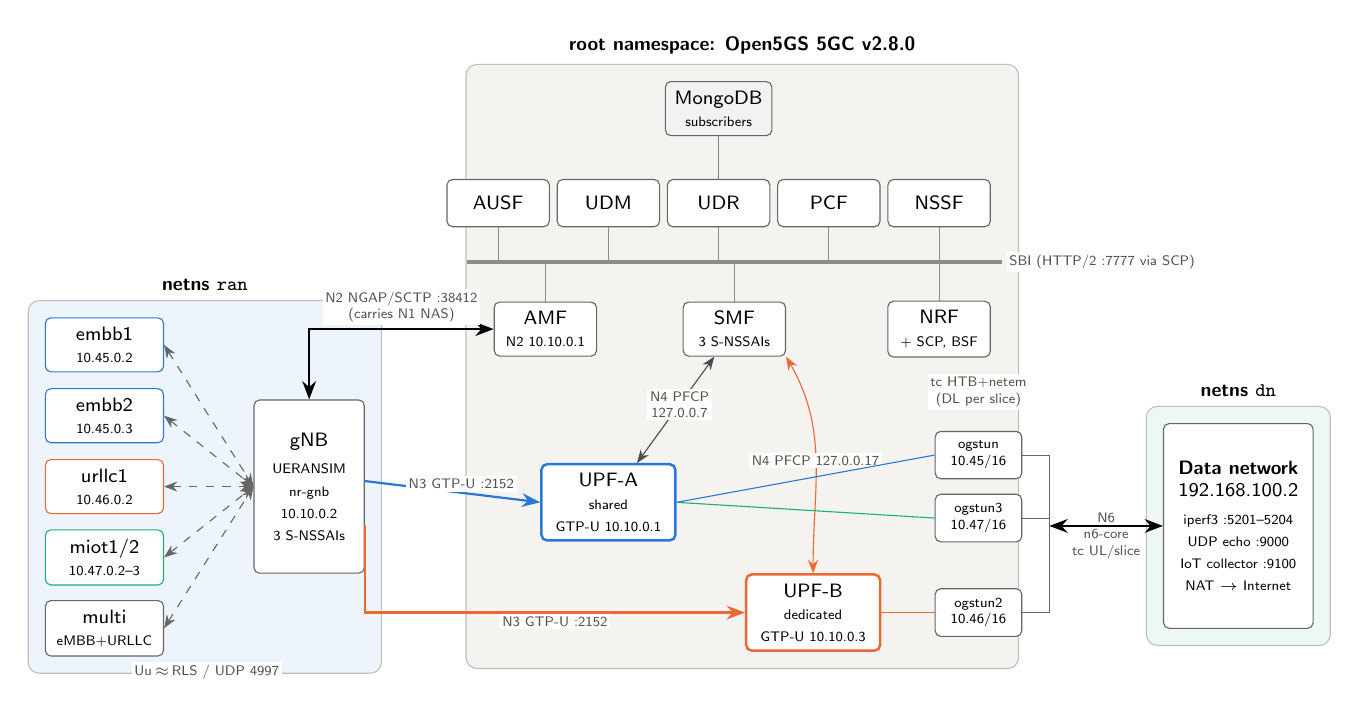
\begin{tikzpicture}[
  font=\sffamily\scriptsize, >=Stealth,
  nf/.style={draw=black!60, rounded corners=2pt, fill=white, minimum width=13mm, minimum height=6mm, align=center},
  ue/.style={nf, minimum width=15mm},
  upf/.style={nf, minimum width=17mm, minimum height=8mm, line width=0.9pt},
  lbl/.style={font=\sffamily\tiny, fill=white, inner sep=1pt, text=ink2, align=center},
  dom/.style={draw=black!25, rounded corners=4pt, inner sep=6pt}]
% ---------------- RAN namespace
\node[ue, draw=embb] (u1) at (0,3.2) {embb1\\\tiny 10.45.0.2};
\node[ue, draw=embb] (u2) at (0,2.3) {embb2\\\tiny 10.45.0.3};
\node[ue, draw=urllc] (u3) at (0,1.4) {urllc1\\\tiny 10.46.0.2};
\node[ue, draw=miot] (u4) at (0,0.5) {miot1/2\\\tiny 10.47.0.2--3};
\node[ue] (u5) at (0,-0.4) {multi\\\tiny eMBB+URLLC};
\node[nf, minimum height=22mm, minimum width=14mm] (gnb) at (2.6,1.4) {gNB\\[2pt]\tiny UERANSIM\\\tiny nr-gnb\\\tiny 10.10.0.2\\\tiny 3 S-NSSAIs};
\foreach \u in {u1,u2,u3,u4,u5} \draw[<->, dashed, black!60] (\u.east) -- (gnb.west);
\node[lbl] at (1.3,-0.95) {Uu\,$\approx$\,RLS / UDP 4997};
\begin{scope}[on background layer]
\node[dom, fill=bgran, fit=(u1)(u5)(gnb), label={[font=\sffamily\scriptsize\bfseries]above:netns \texttt{ran}}] (ran) {};
\end{scope}
% ---------------- Core
\node[nf] (amf) at (5.6,3.4) {AMF\\\tiny N2 10.10.0.1};
\node[nf] (smf) at (8.0,3.4) {SMF\\\tiny 3 S-NSSAIs};
\node[nf] (ausf) at (5.0,5.0) {AUSF};
\node[nf] (udm) at (6.4,5.0) {UDM};
\node[nf] (udr) at (7.8,5.0) {UDR};
\node[nf] (pcf) at (9.2,5.0) {PCF};
\node[nf] (nssf) at (10.6,5.0) {NSSF};
\node[nf] (nrf) at (10.6,3.4) {NRF\\\tiny + SCP, BSF};
\node[nf, fill=black!5] (db) at (7.8,6.2) {MongoDB\\\tiny subscribers};
\draw[black!50] (udr) -- (db);
\draw[black!45, line width=1.4pt] (4.6,4.25) -- (11.4,4.25);
\node[lbl, anchor=west] at (11.45,4.25) {SBI (HTTP/2 :7777 via SCP)};
\foreach \n in {ausf,udm,udr,pcf,nssf} \draw[black!45] (\n.south) -- (\n.south |- 0,4.25);
\foreach \n in {amf,smf,nrf} \draw[black!45] (\n.north) -- (\n.north |- 0,4.25);
\node[upf, draw=embb] (upfa) at (6.4,1.2) {UPF-A\\\tiny shared\\\tiny GTP-U 10.10.0.1};
\node[upf, draw=urllc] (upfb) at (9.0,-0.2) {UPF-B\\\tiny dedicated\\\tiny GTP-U 10.10.0.3};
\draw[<->, black!70] (smf) -- node[lbl, pos=0.45] {N4 PFCP\\127.0.0.7} (upfa);
\draw[<->, urllc] (smf.south east) to[out=-60, in=90] node[lbl, pos=0.5] {N4 PFCP 127.0.0.17} (upfb.north);
% N1/N2/N3
\draw[<->, thick] (gnb.north) |- node[lbl, pos=0.75, above=1pt] {N2 NGAP/SCTP :38412\\(carries N1 NAS)} (amf.west);
\draw[->, thick, embb] ([yshift=2pt]gnb.east) -- node[lbl, pos=0.55, above] {N3 GTP-U :2152} (upfa.west);
\draw[->, thick, urllc] ([yshift=-14pt]gnb.east) |- node[lbl, pos=0.75, below] {N3 GTP-U :2152} (upfb.west);
\begin{scope}[on background layer]
\node[dom, fill=bgcore, fit=(amf)(db)(nssf)(upfa)(upfb)(nrf), inner xsep=10pt,
  label={[font=\sffamily\scriptsize\bfseries]above:root namespace: Open5GS 5GC v2.8.0}] (core) {};
\end{scope}
% ---------------- tun + DN
\node[nf, minimum width=11mm, font=\sffamily\tiny] (t1) at (11.1,1.8) {ogstun\\10.45/16};
\node[nf, minimum width=11mm, font=\sffamily\tiny] (t3) at (11.1,1.0) {ogstun3\\10.47/16};
\node[nf, minimum width=11mm, font=\sffamily\tiny] (t2) at (11.1,-0.2) {ogstun2\\10.46/16};
\draw[embb] (upfa.east) -- (t1.west); \draw[miot] (upfa.east) -- (t3.west); \draw[urllc] (upfb.east) -- (t2.west);
\node[lbl, align=center] at (11.1,2.6) {tc HTB+netem\\(DL per slice)};
\node[nf, minimum height=26mm, minimum width=19mm, align=center] (dn) at (14.4,0.9)
  {\textbf{Data network}\\192.168.100.2\\[2pt]\tiny iperf3 :5201--5204\\\tiny UDP echo :9000\\\tiny IoT collector :9100\\\tiny NAT $\rightarrow$ Internet};
\draw[<->, thick] (12.0,0.9) -- node[lbl, above] {N6} node[lbl, below, align=center] {n6-core\\tc UL/slice} (dn.west);
\foreach \tn in {t1,t2,t3} \draw[black!60] (\tn.east) -- (\tn.east -| 12.0,0) -- (12.0,0.9);
\begin{scope}[on background layer]
\node[dom, fill=bgdn, fit=(dn), label={[font=\sffamily\scriptsize\bfseries]above:netns \texttt{dn}}] {};
\end{scope}
\end{tikzpicture}}
\caption{Deployed end-to-end architecture with all interfaces labelled. The colour of each
user-plane path matches the slice colour used in all plots (\slice{eMBB} blue, \slice{URLLC}
orange, \slice{mIoT} green). Everything runs inside one Ubuntu VM on the Mac host.}
\label{fig:arch}
\end{figure}

\paragraph{Interfaces.} \textbf{Uu} is replaced by UERANSIM's \emph{Radio Link Simulation}
(RLS): RRC/NAS and user data travel between \code{nr-ue} and \code{nr-gnb} as UDP datagrams on
port 4997. That is the channel-simulation mode used in place of radio hardware. It has no PHY,
no MAC scheduling and no fading; \S\ref{sec:limits} covers what that implies.
\textbf{N1} (NAS-5GS) rides inside NGAP. \textbf{N2} is NGAP over SCTP (gNB 10.10.0.2
$\rightarrow$ AMF 10.10.0.1:38412). \textbf{N3} is GTP-U over UDP 2152, terminating at
10.10.0.1 (UPF-A) or 10.10.0.3 (UPF-B). The SMF chooses the UPF per PDU session, and the
choice reaches the gNB as the UL tunnel address in PDUSessionResourceSetupRequest.
\textbf{N4} is PFCP between the SMF (127.0.0.4) and each UPF. \textbf{N6} is the veth to the
\code{dn} namespace. The service-based interfaces (\textbf{N8, N10, N11, N12, N13, N15, N22},
Nnrf, Nbsf) are HTTP/2 on port 7777, using indirect communication through the SCP.

\paragraph{End-to-end path of one URLLC packet.} The \code{urllc\_probe} sends from 10.46.0.2
on \code{uesimtun2} in \code{ran}. \code{nr-ue} carries it over RLS to \code{nr-gnb}, which
encapsulates it in GTP-U (TEID from the PDU session) towards 10.10.0.3. UPF-B decapsulates and
writes it to \code{ogstun2}; the kernel then routes it over \code{n6-core} (tc class 1:20)
into \code{dn}, where the echo server replies. The reply follows the same path in reverse:
\code{ogstun2} egress (tc HTB/netem) $\rightarrow$ UPF-B $\rightarrow$ GTP-U $\rightarrow$
gNB $\rightarrow$ RLS $\rightarrow$ UE.

\section{Implementation by component}\label{sec:impl}
Each component has a named owner who configured it and validated it on its own before
integration (Table~\ref{tab:owners}). All configuration, scripts, sandbox and analysis code
are in the shared repository, \repolink, whose \code{README.md} gives the step-by-step setup
for both platforms. The whole testbed is rebuilt from a clean Mac (Lima) or Windows PC (WSL2)
with the same five scripts.

\begin{table}[H]\centering\small
\caption{Component ownership, deliverables and individual validation evidence.}\label{tab:owners}
\begin{tabularx}{\linewidth}{>{\raggedright}p{2.6cm}>{\raggedright}p{2.6cm}>{\raggedright}X>{\raggedright\arraybackslash}X}
\toprule
Component & Owner & Main artefacts & Individual validation\\
\midrule
Core -- control plane & \memberA & \code{amf, smf, nssf, nrf, ausf, udm, udr, pcf, bsf, scp .yaml}; \code{20\_core.sh} & all NFs register at NRF; NG Setup accepted; Allowed NSSAI in Registration Accept\\
Core -- user plane & \memberB & \code{upf-a.yaml}, \code{upf-b.yaml}, SMF UPF selection, \code{10\_netns.sh} (N3/N6, tun, NAT) & PFCP association with both UPFs; PFCP Session Establishment to the right UPF per DNN\\
Radio access network & \memberC & \code{gnb.yaml}, RAN namespace, \code{40\_ran.sh} & SCTP association + NGSetupResponse; per-UE PDUSessionResourceSetup\\
UE \& provisioning & \memberD & \code{gen\_ues.sh} (7 UE configs), \code{30\_subscribers.sh}, \code{ue\_cfg.py}, \code{ue\_table.sh} & 6 UEs RM-REGISTERED with 7 PDU sessions; negative UE rejected\\
Traffic generation & \memberE & \code{embb.py}, \code{urllc\_probe.py}, \code{miot\_client.py}, DN servers & per-slice KPI CSVs; on/off, periodic and Poisson profiles verified (Fig.~\ref{fig:e6})\\
Signalling analysis & \memberF & \code{50\_capture.sh}, \code{analysis/analyze.py} & decoded call flow, timing and SBI tables (\S\ref{sec:e2})\\
Sandbox application & \memberG & \code{sandbox/app.py}, \code{testbed.py}, \code{slice\_ctl.sh} & every control exercised from the UI (\S\ref{sec:sandbox})\\
Platform \& integration & \memberH & \code{vm/lima-5g.yaml}, \code{vm/wslconfig.example}, \code{wsl\_setup.sh}, \code{00\_provision.sh}, \code{experiments/run\_all.py}, \code{versions.sh} & clean rebuild; scripted E1--E7; Windows checks\\
\bottomrule
\end{tabularx}
\end{table}

\subsection{Core network -- control plane (\memberA)}
Open5GS~2.8.0~\cite{open5gs} was installed from the project's PPA (arm64 build on the Mac; the same PPA ships amd64 for Windows PCs). The NFs are
not run as the packaged systemd units. \code{20\_core.sh} starts them in dependency order
(NRF $\rightarrow$ SCP $\rightarrow$ AUSF/UDM/UDR/PCF/NSSF/BSF $\rightarrow$ UPFs
$\rightarrow$ SMF $\rightarrow$ AMF) from the repository configs, so that every parameter is
under version control. The configs deviate from the defaults as follows. The PLMN is changed
to the test PLMN 001/01. The AMF binds NGAP to 10.10.0.1 and supports three S-NSSAIs. Its
integrity order is NIA2$>$NIA1 and its ciphering order is \emph{NEA0 first}, so NAS stays
readable in captures (the integrity protection is still checked). The NSSF has one NSI per
S-NSSAI, and the SMF advertises \code{info.s\_nssai} for all three slices. MongoDB~8.0 holds
the subscriber records.

\subsection{Core network -- user plane (\memberB)}
Two \code{open5gs-upfd} instances run with separate PFCP (127.0.0.7 / 127.0.0.17), GTP-U
(10.10.0.1 / 10.10.0.3) and metrics addresses. The SMF selects the UPF by DNN
(\code{pfcp.client.upf[].dnn}). A second SMF/UPF-A configuration pair (\code{smf-shared.yaml},
\code{upf-a-shared.yaml}) puts URLLC on UPF-A for the shared-UPF experiment. Pool addressing
lives in both the SMF and the UPF \code{session} lists, with an explicit \code{dev} so that
each DNN uses its own tun device. \code{10\_netns.sh} creates the tun devices persistently, so
the tc qdiscs survive UPF restarts. It also sets the DN return routes and the NAT.

\subsection{Radio access network (\memberC)}
UERANSIM~v3.2.7~\cite{ueransim} was built from source (gcc~13.3, CMake~3.28). The gNB
(\code{nci 0x10}, TAC~1, 32-bit gNB-ID) runs in the \code{ran} namespace. It binds its RLS
side to 127.0.0.1 and its N2/N3 side to 10.10.0.2. It lists all three S-NSSAIs; without
this, the AMF would reject NG Setup for unsupported slices. \code{ignoreStreamIds} works
around Open5GS's SCTP stream allocation.

\subsection{User equipment and provisioning (\memberD)}
\code{gen\_ues.sh} writes one UE config per subscriber from a single template, which avoids
copy-paste drift. Each config holds the SUPI, K, OPc, null-scheme SUCI, the sessions (DNN +
S-NSSAI), the configured/default NSSAI and the algorithms. \code{30\_subscribers.sh} creates
the matching UDR records with \code{open5gs-dbctl} and then writes the per-slice QoS profile
(5QI, ARP, Session-AMBR) into each session with \code{mongosh}. Seven subscribers exist: two
eMBB, one URLLC, two mIoT gateways, one \emph{multi-slice} UE subscribed to eMBB+URLLC (it
holds two concurrent PDU sessions on two UPFs), and one negative-test UE subscribed only to
eMBB that requests URLLC. At start-up \code{ue\_cfg.py} derives each UE's runtime config,
keeping only the sessions of slices that are administratively up (\S\ref{sec:sandbox}).

\subsection{Traffic generation (\memberE)}\label{sec:traffic}
Each service class has a generator that matches its temporal profile. All generators write one
KPI row per second (\code{traffic/kpi.py}) and bind to the UE's PDU-session address, so all
traffic enters the 5G user plane.
\begin{itemize}
\item \textbf{eMBB} (\code{embb.py}): wraps iperf3~3.16~\cite{iperf3} in reverse (downlink)
  mode with $N$ parallel TCP streams in an on/off cycle (default 20\,s/5\,s). It parses the
  per-second rate and logs explicit zeros during off periods.
\item \textbf{URLLC} (\code{urllc\_probe.py}): sends sequence-numbered, timestamped 64-byte
  UDP packets at a fixed rate (100\,Hz by default) to the DN echo server. It uses
  \code{select()} so that echoes are timestamped on arrival, and reports per-second RTT p50,
  p99, jitter (mean $|\Delta\text{RTT}|$) and loss (no echo within 1\,s).
\item \textbf{mIoT} (\code{miot\_client.py}): simulates $D$ sensors behind one gateway UE. Each
  sends a JSON report with exponential inter-arrival times (mean $P$); the collector returns a
  16-byte ACK. It reports reports/s, ACK latency and loss (no ACK within 2\,s).
\end{itemize}

\subsection{Signalling capture and analysis (\memberF)}
\code{50\_capture.sh} runs \code{tshark} on \code{n3-core} (N2, N3) and \code{lo} (SBI, N4).
The capture filter is SCTP, UDP 2152/8805 and TCP 7777. \code{analysis/analyze.py} decodes it
with \code{nas-5gs.null\_decipher} and \code{-d tcp.port==7777,http2}. It extracts per-UE
procedure timing (keyed on RAN-UE-NGAP-ID and SUCI MSIN), PFCP sessions per UPF and SBI
operations. It also draws the message ladder and every KPI figure from the CSVs.

\subsection{Sandbox application (\memberG)}
The sandbox has three layers, so the user interface never touches the testbed directly:
\begin{itemize}
\item \textbf{UI} (\code{sandbox/app.py}, Streamlit). It renders the slice cards, the live
  parameter forms, the KPI charts, the UE/PDU-session table and the event log. The KPI panel
  is a fragment that re-runs every 2\,s, so only the charts refresh while the rest of the
  page stays still.
\item \textbf{Control library} (\code{sandbox/testbed.py}). It exposes the actions: apply a
  scenario, slice up/down, start/stop traffic, set QoS, read KPIs and export a run. It starts
  traffic generators in the \code{ran} namespace as separate process groups bound to each
  UE's current PDU address, so ``stop'' always removes every child process. Every action is
  appended to the run's \code{events.csv}.
\item \textbf{Slice control} (\code{scripts/slice\_ctl.sh}). It applies the tc HTB/netem
  changes and the deregister/re-attach cycle for slice up/down. Administrative state lives in
  files under \code{/run/e2e5g}, so a page reload or a second browser sees the same state.
\end{itemize}
The experiment runner uses the same library, so every sandbox action can be reproduced by
script. Section~\ref{sec:sandbox} shows the resulting interface.

\subsection{Platform and integration (\memberH)}
Every script assumes the repository at \code{/e2e5g} and an Ubuntu~24.04 environment, so
the host only has to provide those two things. On macOS, \code{vm/lima-5g.yaml} defines the
VM, mounts the repository at \code{/e2e5g} (virtiofs) and forwards port 8501 (sandbox) to the
Mac. On Windows, WSL2 runs Ubuntu~24.04 with the resources in \code{vm/wslconfig.example}, and
\code{scripts/wsl\_setup.sh} prepares it. The script enables systemd, links the clone to
\code{/e2e5g} and rejects CRLF line endings. It also live-tests every kernel feature the
testbed needs (SCTP sockets, netns, veth, TUN, tc HTB and netem) before anything is
installed. \code{00\_provision.sh} is idempotent, detects the CPU architecture (arm64 or
amd64) and installs every dependency on either platform. \code{experiments/run\_all.py} restarts the testbed into a known
state before each experiment and drives the same \code{testbed.py} API that the sandbox uses,
so demo and measurements share one code path. \code{versions.sh} records the exact version of every
component in \code{results/versions.txt} (Open5GS 2.8.0, MongoDB 8.0.32, UERANSIM v3.2.7,
iperf3 3.16, TShark 4.2.2, iproute2 6.1.0, Python 3.12.3, Streamlit 1.65.0; guest Ubuntu
24.04.5 with kernel 6.8.0; host macOS 27.0 with Lima 2.2.1).

\section{Sandbox application}\label{sec:sandbox}
The sandbox (\code{sandbox/app.py}, Streamlit~1.65~\cite{streamlit}) is the single control
surface for someone who did not build the system. It runs as root inside the VM and is
opened in a browser on the host (Mac or Windows) at \url{http://localhost:8501}. Its controls map one-to-one onto the
required capabilities (Table~\ref{tab:sandbox}). Every action goes through
\code{sandbox/testbed.py}. That is the same library the scripted experiments use, so a result
seen in the demo can be reproduced exactly by script. Every action is also appended to the
run's \code{events.csv}, which later annotates the plots.

\begin{table}[H]\centering\small
\caption{Sandbox capabilities and how each is realised in the testbed.}\label{tab:sandbox}
\begin{tabularx}{\linewidth}{>{\raggedright}p{3.2cm}>{\raggedright}p{3.6cm}>{\raggedright\arraybackslash}X}
\toprule
Requirement & UI control & Mechanism\\
\midrule
Select a scenario & sidebar: \emph{Service scenario} + \emph{Apply} & preset of per-slice tc parameters + traffic profiles (S1 baseline, S2 factory peak, S3 degraded transport, S4 massive-IoT burst)\\
Bring slices up/down & per-slice \emph{Slice up / Slice down} & switch-off deregistration of the slice's UEs, then re-attach with a runtime config without (or with) that S-NSSAI; multi-slice UEs keep their other session\\
Start/stop traffic per slice & \emph{Start / Stop traffic} & generator processes in the \code{ran} netns bound to the UE's current PDU address (process groups, so stop is clean)\\
Change a slice parameter live & \emph{Live slice parameters} form (MBR, delay, loss) & \code{tc class change} (HTB rate) and \code{tc qdisc change} (netem) on DL tun + UL N6 class; no session impact\\
View live per-slice KPIs & metrics + charts, auto-refresh 2\,s & 1-s KPI rows aggregated per slice: throughput, RTT p50/p99, loss\\
Export run data & \emph{Export run (ZIP)} & KPI CSVs, event log, UE/PDU table, current QoS\\
\bottomrule
\end{tabularx}
\end{table}

\begin{figure}[!htbp]\centering
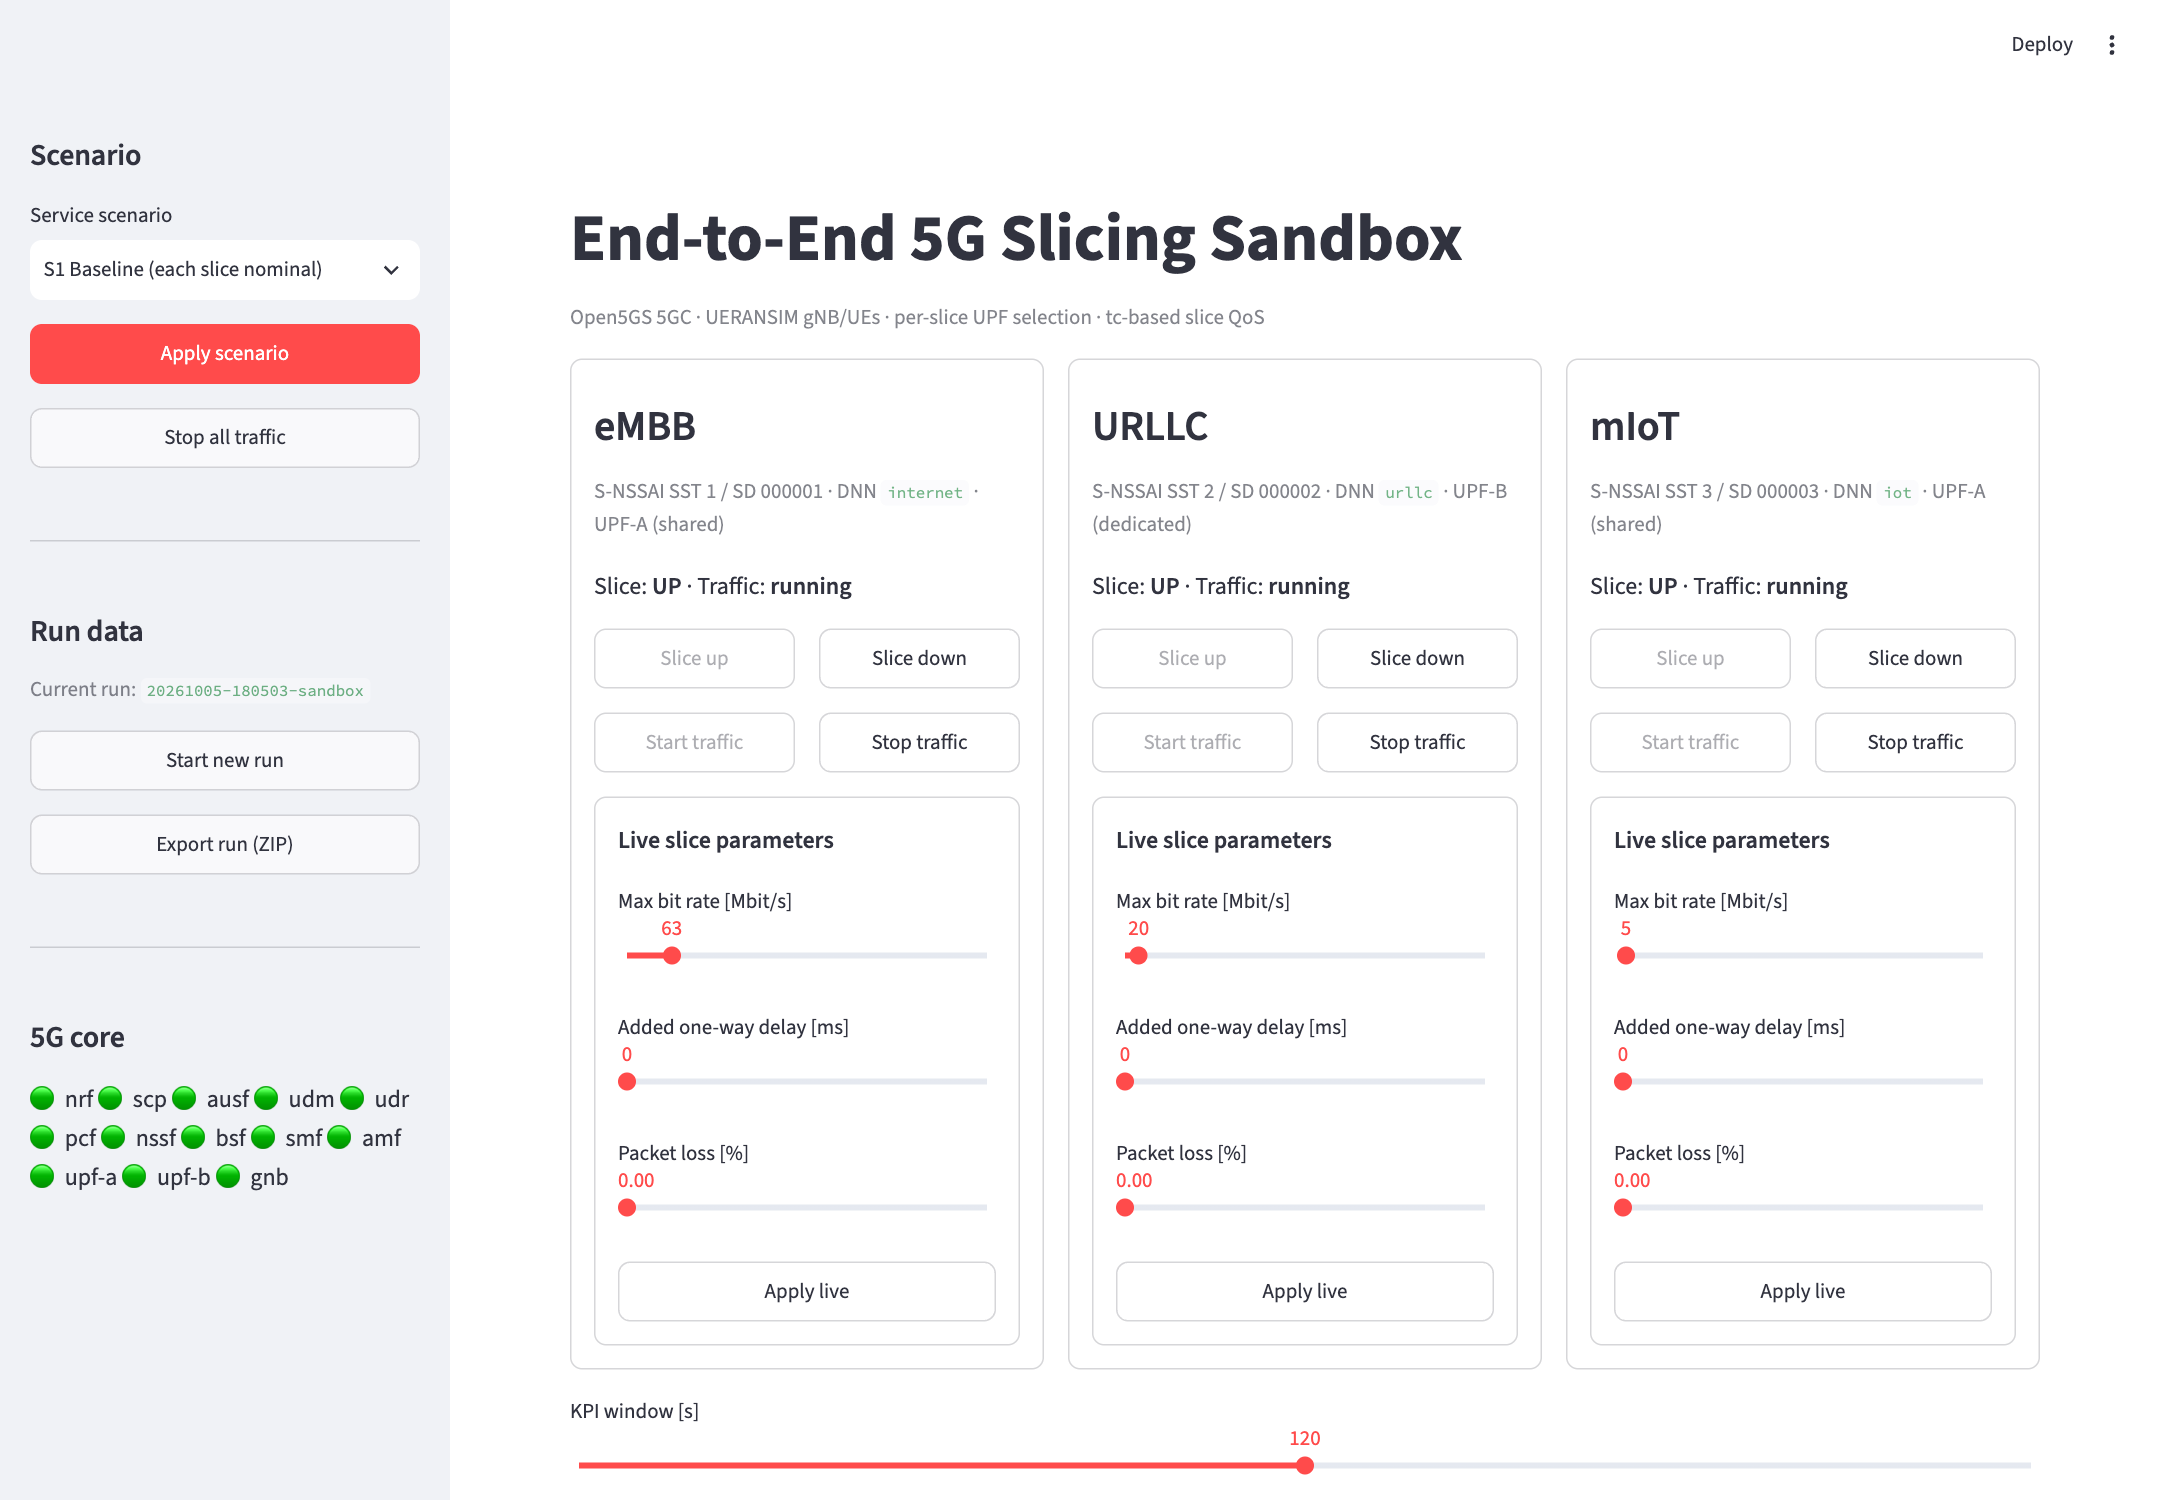
\includegraphics[width=0.86\linewidth]{screenshots/sandbox_top.png}
\caption{Sandbox during scenario S1. Each slice card shows its S-NSSAI, DNN and UPF, its admin
and traffic state, and the live parameter form. The 5GC NF health is shown in the sidebar.}
\label{fig:sandbox1}
\end{figure}
\begin{figure}[!htbp]\centering
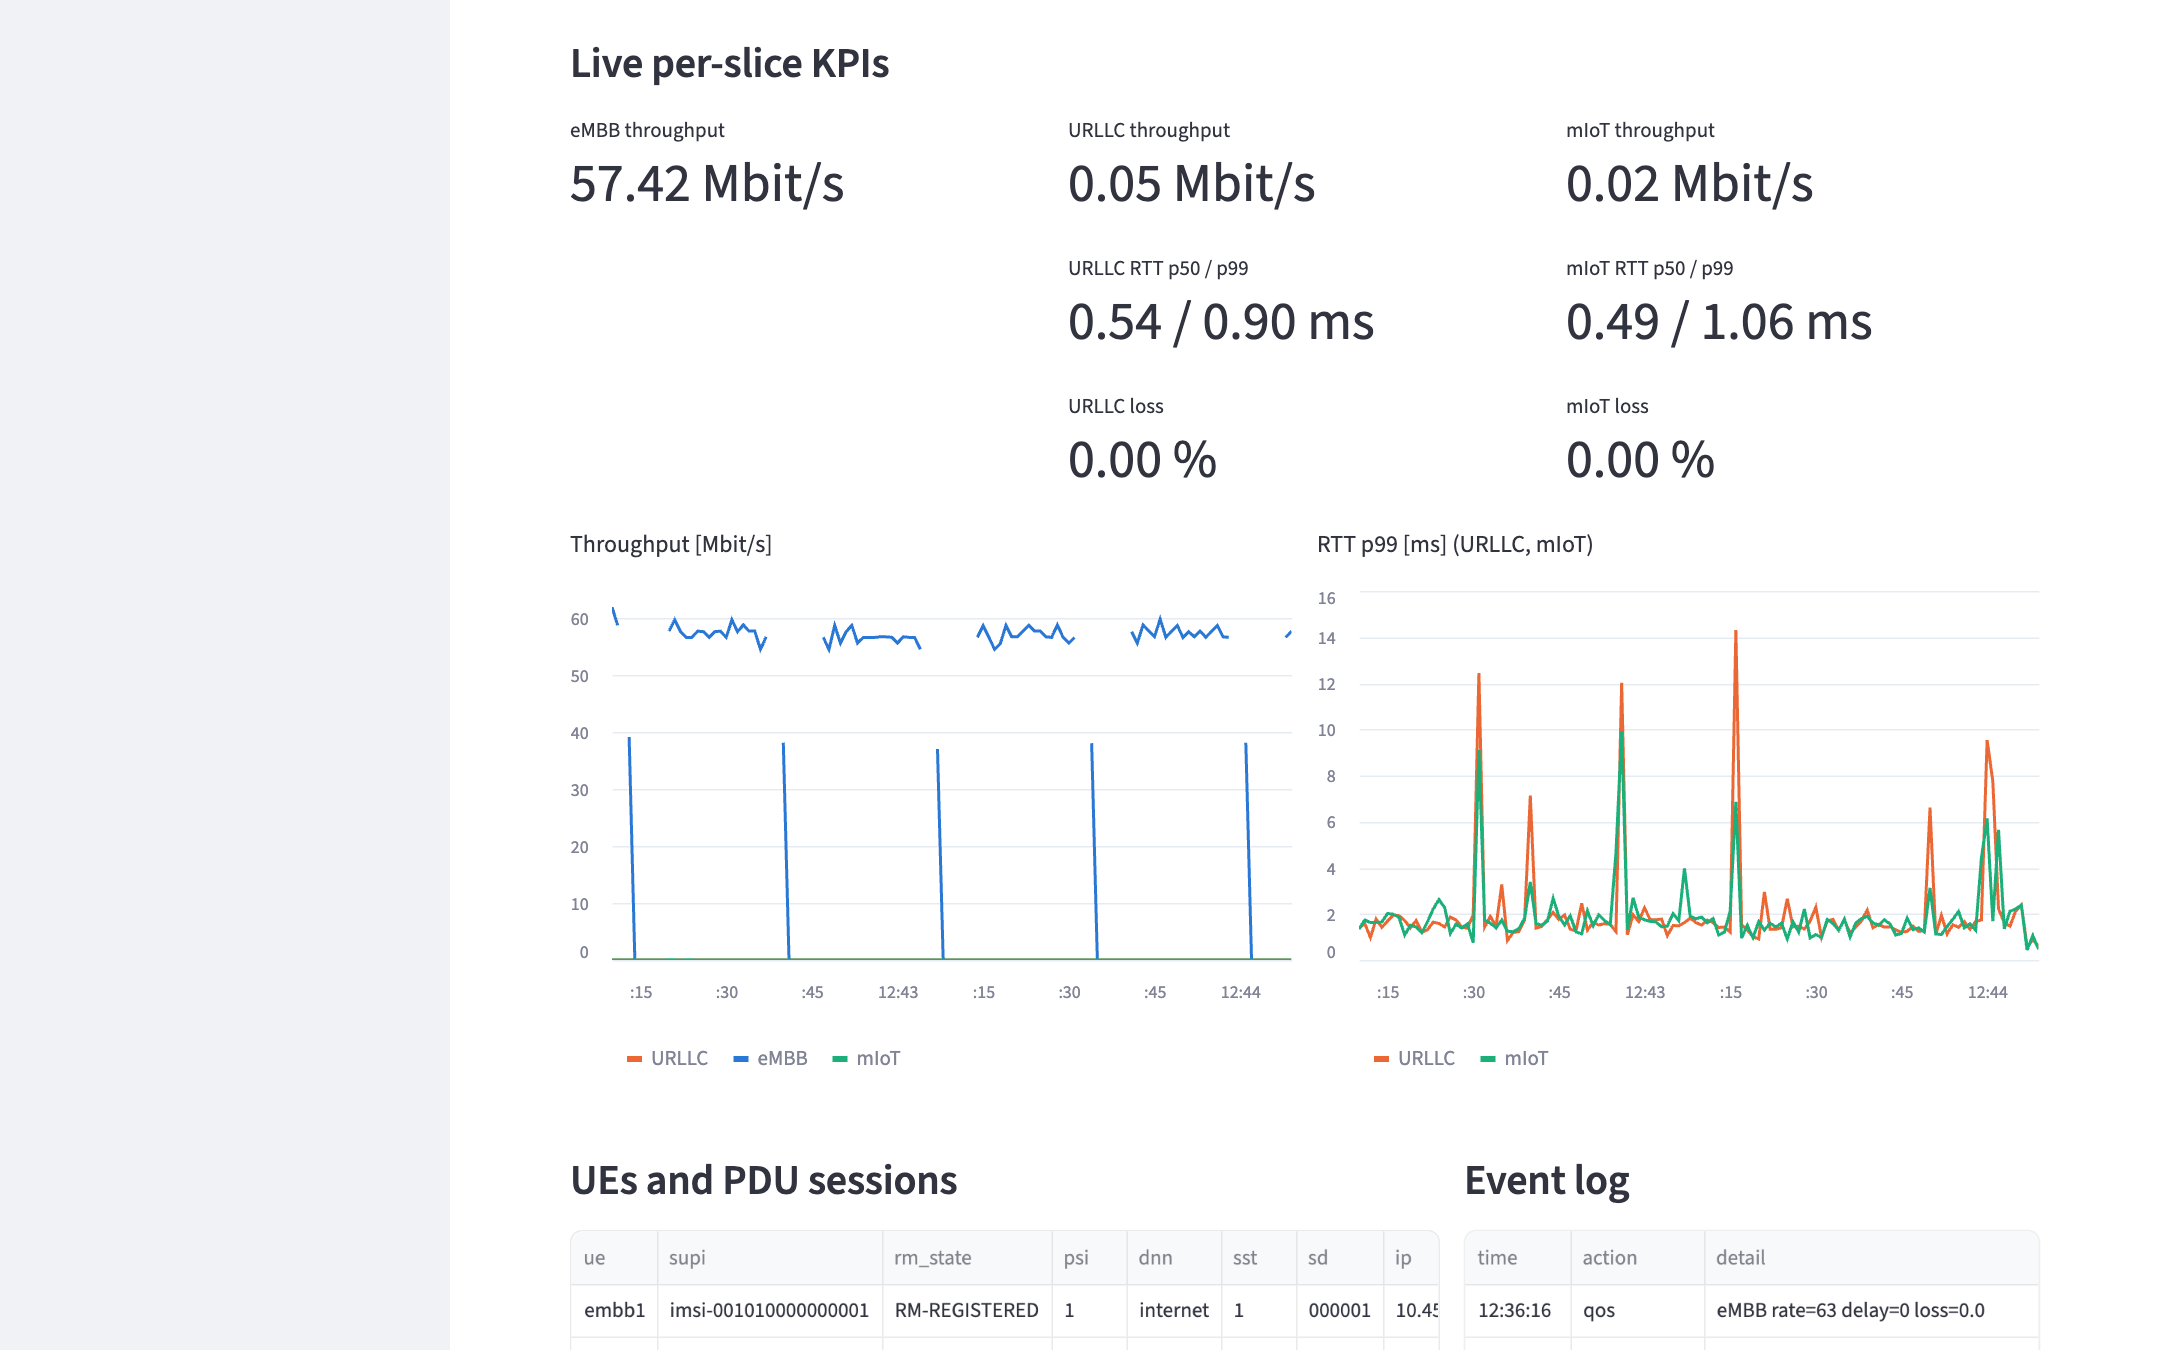
\includegraphics[width=0.86\linewidth]{screenshots/sandbox_kpis.png}
\caption{Sandbox live KPI panel, UE/PDU-session table and event log after a live change of the
eMBB MBR.}\label{fig:sandbox2}
\end{figure}

\paragraph{Design decision: slice down.} Our first implementation released the slice's PDU
sessions with \code{nr-cli ps-release}. UERANSIM, however, re-establishes every session listed
in its config within $\approx$200\,ms, so the slice came straight back (with new addresses).
The final design treats ``slice down'' as an administrative state
(\code{/run/e2e5g/state-<slice>}). The affected UEs perform a switch-off deregistration, which
makes the AMF/SMF release all their contexts and PFCP sessions. They then re-attach from a
runtime config filtered to the slices that are still up. This also exercises the
deregistration and re-registration procedures on demand.

\section{Experimental method}\label{sec:method}
Every experiment is scripted in \code{experiments/run\_all.py} and starts from a known state:
RAN stopped, core restarted, slice qdiscs reset to Table~\ref{tab:slices}, and DN services
restarted. The traffic generators log one KPI sample per second per UE. The analysis
aggregates per slice and per second: throughput is summed over UEs, p50 is averaged, and p99
takes the worst UE. Phase boundaries come from the event log. The experiments follow one
thread: \emph{does each slice meet its Table~\ref{tab:req} target on its own, under
cross-slice load, after live re-parameterisation, and with or without a dedicated user plane?}

\begin{table}[!htbp]\centering\small
\caption{Experiment plan.}\label{tab:exp}
\begin{tabularx}{\linewidth}{l>{\raggedright}p{3.4cm}>{\raggedright}X>{\raggedright\arraybackslash}p{3.1cm}}
\toprule
ID & Question & Procedure & Output\\
\midrule
E1 & Do all UEs register, get the right slice/IP/UPF, and reach the DN? & capture on; start gNB + 6 UEs + negative UE; ping (10$\times$) from every PDU session; iperf3 5\,s and HTTP per slice & UE table, pcap, ping/iperf logs\\
E2 & Is registration, session establishment and slice selection visible in signalling? & decode the E1 pcap (NGAP/NAS/PFCP/SBI) & ladder, timing, SBI tables\\
E3 & Is URLLC/mIoT isolated from an eMBB surge? & URLLC 100\,Hz + mIoT 2$\times$500 devices for 120\,s; eMBB 2 UEs $\times$4 TCP streams in $t$=30--90\,s & RTT/loss by phase\\
E4 & Do live slice-parameter changes take effect, and only on that slice? & all slices active 120\,s; $t$=40\,s eMBB MBR 150$\rightarrow$30\,Mbit/s; $t$=80\,s URLLC +5\,ms each way & time series around changes\\
E5 & Is a dedicated URLLC UPF justified? & 2 runs: dedicated (UPF-B) vs shared (UPF-A); URLLC 200\,Hz; eMBB cap removed, 2 UEs $\times$8 streams in $t$=20--80\,s & RTT p99 series + CDF\\
E6 & Do generators reproduce the temporal profiles? & scenario S1 for 90\,s & per-slice profiles\\
\bottomrule
\end{tabularx}
\end{table}

\paragraph{Metrics.} RTT is measured end-to-end, UE$\leftrightarrow$DN, through RLS, gNB,
GTP-U, UPF, tc and N6. One-way delays cannot be measured reliably because there is no shared
clock across processes (\S\ref{sec:limits}). Throughput is the iperf3 receiver goodput at the
UE. Loss is a missing echo/ACK after 1\,s/2\,s. Signalling latencies come from capture
timestamps on \code{n3-core}.

\section{Results}\label{sec:results}
All numbers below come from the runs stored in \code{results/} and were produced by
\code{analysis/analyze.py}. Nothing was edited by hand.

\subsection{E1 -- Deployment and UE-to-data-network connectivity}\label{sec:e1}
All twelve 5GC processes and the gNB started; the NG Setup succeeded
(\code{gNB-N2 accepted[10.10.0.2]}, \code{Number of gNBs is now 1}), and the SMF formed PFCP
associations with both UPFs. Listing~\ref{lst:uetable} is the state reported by
\code{nr-cli} after attach. Every UE is \code{RM-REGISTERED}. The multi-slice UE holds
\emph{two} PDU sessions in two pools (10.45.0.4 on eMBB, 10.46.0.3 on URLLC). The negative
test UE \code{badslice} registers but obtains no address.

\begin{lstlisting}[caption={UE and PDU-session state after E1 attach (\code{results/e1/ue\_table.txt}).},label={lst:uetable}]
UE        SUPI                  RM-STATE       PSI  DNN       SST  SD      ADDRESS      IFACE
badslice  imsi-001010000000007  RM-REGISTERED  1    urllc     2    000002  null         -
embb1     imsi-001010000000001  RM-REGISTERED  1    internet  1    000001  10.45.0.2    uesimtun0
embb2     imsi-001010000000002  RM-REGISTERED  1    internet  1    000001  10.45.0.3    uesimtun1
miot1     imsi-001010000000004  RM-REGISTERED  1    iot       3    000003  10.47.0.2    uesimtun3
miot2     imsi-001010000000005  RM-REGISTERED  1    iot       3    000003  10.47.0.3    uesimtun4
multi     imsi-001010000000006  RM-REGISTERED  1    internet  1    000001  10.45.0.4    uesimtun5
multi     imsi-001010000000006  RM-REGISTERED  2    urllc     2    000002  10.46.0.3    uesimtun6
urllc1    imsi-001010000000003  RM-REGISTERED  1    urllc     2    000002  10.46.0.2    uesimtun2
\end{lstlisting}

\noindent The AMF rejects the unsubscribed slice explicitly, and the UE reports the
corresponding 5GMM cause:
\begin{lstlisting}
[amf] [gmm] WARNING: [imsi-001010000000007] Ue requested DNN "urllc" Not Supported OR Not Subscribed in the Slice
[ue ] [nas] [error] MM status received with cause [DNN_NOT_SUPPORTED_OR_NOT_SUBSCRIBED]
\end{lstlisting}

\paragraph{Data flow.} Every PDU session reached the DN: 10/10 ICMP echoes from each of the
seven sessions, with RTT averages of 0.72--0.93\,ms. The same capture proves that the traffic
used the intended user plane (Listing~\ref{lst:gtpu}). eMBB and mIoT packets are tunnelled
to UPF-A (10.10.0.1), and \emph{both} URLLC sessions (urllc1 and multi's second session) to
UPF-B (10.10.0.3). Each session has its own TEID pair. iperf3 downlink goodput was
138\,Mbit/s on eMBB, 18.7\,Mbit/s on URLLC and 2.10\,Mbit/s on mIoT. These match the binding
cap of each slice: the tc MBR of 150 and 20\,Mbit/s, and the 2\,Mbit/s Session-AMBR for mIoT.
HTTP requests from each slice through N6 and NAT to a public web server returned
\code{200} in 72--80\,ms.

\begin{lstlisting}[caption={GTP-U-encapsulated pings per N3 endpoint, outer$\rightarrow$inner
addresses (\code{results/e1/gtpu\_per\_upf.txt}; uplink rows shown).},label={lst:gtpu}]
 10 10.10.0.2->10.10.0.1  inner 10.45.0.2->192.168.100.2  teid 0x00006eee   eMBB  -> UPF-A
 10 10.10.0.2->10.10.0.1  inner 10.45.0.4->192.168.100.2  teid 0x0000a57f   eMBB  -> UPF-A (multi)
  9 10.10.0.2->10.10.0.3  inner 10.46.0.2->192.168.100.2  teid 0x00000600   URLLC -> UPF-B
 10 10.10.0.2->10.10.0.3  inner 10.46.0.3->192.168.100.2  teid 0x0000f718   URLLC -> UPF-B (multi)
 10 10.10.0.2->10.10.0.1  inner 10.47.0.2->192.168.100.2  teid 0x000044f9   mIoT  -> UPF-A
\end{lstlisting}

\subsection{E2 -- Signalling: registration, session establishment and slice selection}\label{sec:e2}
Figure~\ref{fig:ladder} is the message sequence of the multi-slice UE, reconstructed directly
from the capture. It shows the complete 5G registration (TS~23.502~\S4.2.2.2~\cite{ts23502}).
InitialUEMessage carries the Registration Request with the SUCI and the requested NSSAI. The
AMF fetches 5G-AKA vectors via AUSF/UDM (Authentication Request/Response). The Security Mode
Command then selects NIA2/NEA0. InitialContextSetupRequest carries the Registration Accept,
whose \textbf{Allowed NSSAI} contains exactly the subscribed S-NSSAIs: \code{SST 1/SD 000001} and
\code{SST 2/SD 000002} for this UE.
Table~\ref{tab:nssai} lists the NSSAI each UE received. The UE subscribed only to eMBB that
asked for URLLC gets \code{SST 1} as Allowed NSSAI and \code{SST 2/SD 000002} as
\textbf{Rejected NSSAI} (cause 0, ``S-NSSAI not available in the current PLMN''). That is
exactly the behaviour TS~24.501 specifies for a non-subscribed S-NSSAI~\cite{ts24501}.

\begin{table}[H]\centering\small
\caption{NSSAI in each Registration Accept, decoded from the capture (\code{results/e1/allowed\_nssai.txt}).}\label{tab:nssai}
\begin{tabular}{lll}
\toprule
UE (RAN-UE-NGAP-ID) & Allowed NSSAI (SST/SD) & Rejected NSSAI\\
\midrule
embb1 (1), embb2 (2) & 1/000001 & --\\
urllc1 (3) & 2/000002 & --\\
miot1 (4), miot2 (5) & 3/000003 & --\\
multi (6) & 1/000001, 2/000002 & --\\
badslice (7) & 1/000001 & 2/000002 (cause 0)\\
\bottomrule
\end{tabular}
\end{table}

\noindent Two PDU Session Establishment Requests follow (one per S-NSSAI/DNN). The SMF then opens one
PFCP session on \textbf{UPF-B} (127.0.0.17, URLLC) and one on \textbf{UPF-A} (127.0.0.7,
eMBB), and each N2 PDUSessionResourceSetupRequest gives the gNB the corresponding UPF N3
address.

\begin{figure}[H]\centering
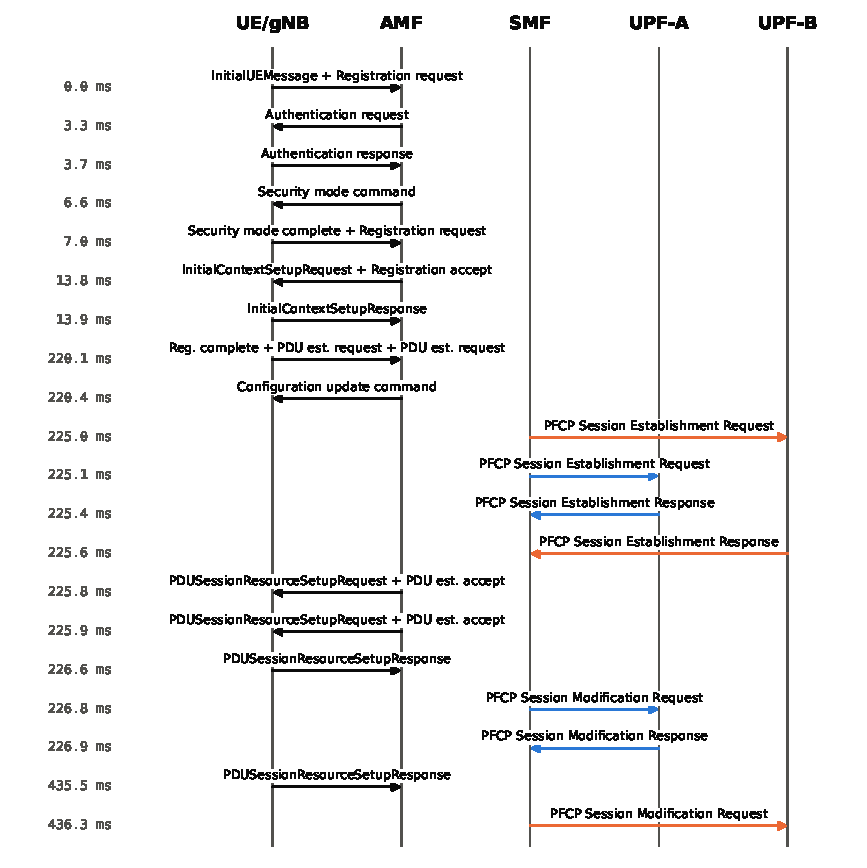
\includegraphics[width=0.76\linewidth]{figures/fig_ladder_multi.pdf}
\caption{N2 (NGAP/NAS) and N4 (PFCP) messages for UE \code{imsi-001010000000006}, extracted from
\code{results/e1/attach.pcapng}. Orange arrows: PFCP to the dedicated URLLC UPF-B; blue: shared
UPF-A. Times are relative to the InitialUEMessage.}\label{fig:ladder}
\end{figure}

Over all UEs the capture contains 5 PFCP Session Establishments towards UPF-A and 2 towards
UPF-B, which is exactly the number of eMBB+mIoT and URLLC sessions. Table~\ref{tab:sigtime}
gives the procedure latencies. Registration completes in 7--17\,ms and a PDU session in
6--15\,ms. The $\approx$200\,ms gap between Registration Accept and the first PDU request is
UERANSIM's own timer, not network latency. Table~\ref{tab:sbi} lists the service-based
operations behind these procedures (N8/N10/N12/N13 UDM/UDR/AUSF, N11 AMF$\rightarrow$SMF,
N7/N15 PCF, BSF binding). Every SBI request is counted twice, because the capture sees both
hops (NF$\rightarrow$SCP$\rightarrow$NF).

\begin{table}[H]\centering\small
\begin{minipage}[t]{0.52\linewidth}\centering
\caption{Procedure latency per UE (from N2 timestamps).}\label{tab:sigtime}
\resizebox{\linewidth}{!}{\begin{tabular}{llrcl}
\toprule
UE & SUPI & Registration [ms] & PDU sessions & PDU setup [ms] \\
\midrule
embb1 & imsi-001010000000001 & 15.3 & 1 & 15.2 \\
embb2 & imsi-001010000000002 & 12.1 & 1 & 9.2 \\
urllc1 & imsi-001010000000003 & 15.5 & 1 & 7.9 \\
miot1 & imsi-001010000000004 & 12.8 & 1 & 10.8 \\
miot2 & imsi-001010000000005 & 7.3 & 1 & 10.4 \\
multi & imsi-001010000000006 & 13.8 & 2 & 6.4, 215.4 \\
badslice & imsi-001010000000007 & 17.0 & 0 & rejected \\
\bottomrule
\end{tabular}
}
\end{minipage}\hfill
\begin{minipage}[t]{0.45\linewidth}\centering
\caption{Most frequent SBI operations (excluding NRF heartbeats).}\label{tab:sbi}
\resizebox{\linewidth}{!}{\begin{tabular}{llr}
\toprule
SBI API & Operation & Count \\
\midrule
nudr-dr & GET /subscription-data/\{supi\} & 56 \\
nudr-dr & GET /policy-data/ues & 28 \\
nudm-sdm & POST /\{supi\}/sdm-subscriptions & 28 \\
nudr-dr & PUT /subscription-data/\{supi\} & 27 \\
nudm-uecm & PUT /\{supi\}/registrations & 22 \\
nsmf-pdusession & POST /sm-contexts & 14 \\
nsmf-pdusession & POST /sm-contexts/\{id\} & 14 \\
namf-comm & POST /ue-contexts/\{supi\} & 14 \\
nbsf-management & POST /pcfBindings & 14 \\
npcf-smpolicycontrol & POST /sm-policies & 14 \\
nudm-sdm & GET /\{supi\}/sm-data & 14 \\
nausf-auth & POST /ue-authentications & 14 \\
\bottomrule
\end{tabular}
}
\end{minipage}
\end{table}

\subsection{E6 -- Temporal traffic profiles per slice}
Figure~\ref{fig:e6} confirms that each generator reproduces its service class (scenario S1,
90\,s). eMBB alternates 20\,s downloads at the 150\,Mbit/s slice cap (two UEs share it) with
5\,s idle gaps. URLLC is a perfectly periodic 100 echoes/s at 0.05\,Mbit/s. mIoT shows the
Poisson-modulated arrival of 400 sensors (mean 38 reports/s for 200 devices $\times$ 2 gateways
at a 10\,s mean period; theory 40/s).

\begin{figure}[H]\centering
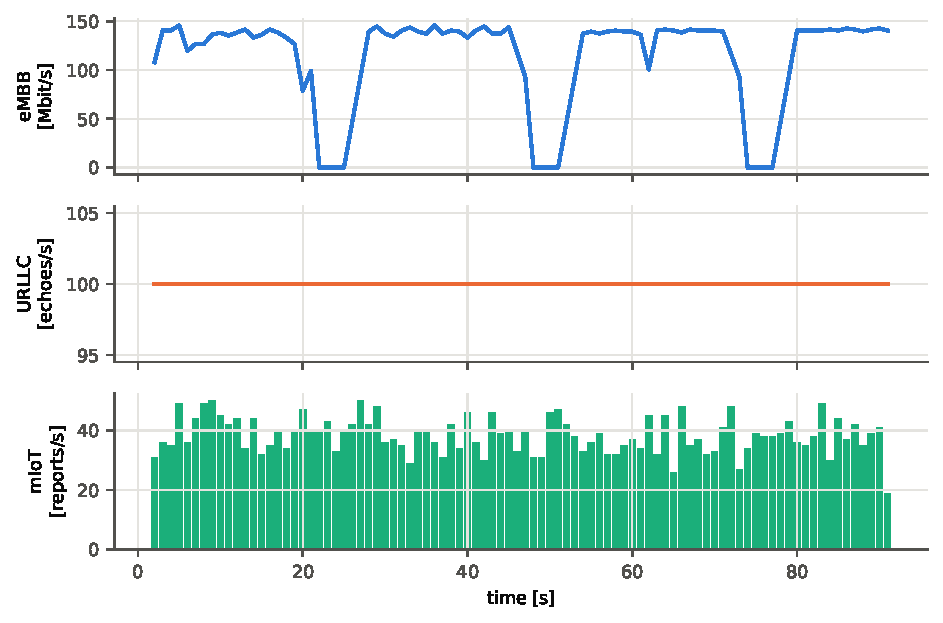
\includegraphics[width=0.74\linewidth]{figures/fig_e6_profiles.pdf}
\caption{Per-slice offered traffic in scenario S1 (E6).}\label{fig:e6}
\end{figure}

\subsection{E3 -- Isolation of URLLC and mIoT from an eMBB surge}\label{sec:e3}
Figure~\ref{fig:e3} and Table~\ref{tab:e3} show URLLC and mIoT latency before, during and
after an eMBB surge of 2 UEs $\times$ 4 TCP streams. The surge is held at the eMBB slice MBR
($\approx$141\,Mbit/s mean). Neither slice lost a single packet, and their p99 stayed below
1.1\,ms throughout the load phase. The URLLC p99 target of Table~\ref{tab:req} (10\,ms) was
met in every per-second window of the load phase (worst 1.43\,ms). The only violations were
isolated spikes of 13--19\,ms in the \emph{idle} phases. Latency is visibly \emph{lower} under
load (p50 0.32 vs.\ 1.08\,ms). Control experiment E7 explains this (Table~\ref{tab:e7}): pure
CPU busy-loops with no network traffic lower the URLLC p50 from 1.08 to 0.10\,ms. The idle
penalty is therefore CPU idle-state wake-up latency in the VM, not a property of the 5G
stack.

\begin{figure}[H]\centering
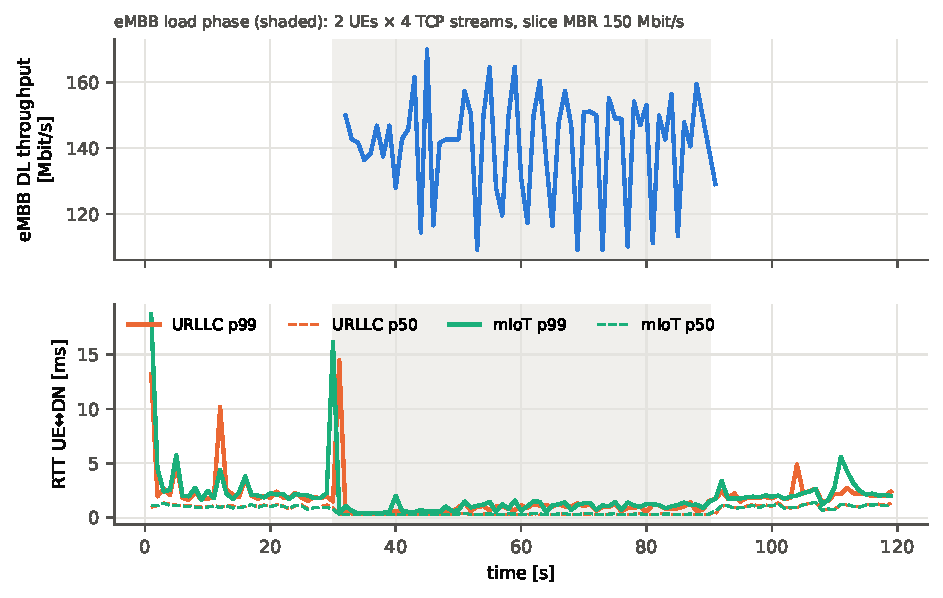
\includegraphics[width=0.78\linewidth]{figures/fig_e3_isolation.pdf}
\caption{E3: eMBB surge (top) and URLLC/mIoT RTT (bottom). Shaded: eMBB load phase.}\label{fig:e3}
\end{figure}

\begin{table}[H]\centering\small
\caption{E3 latency by phase (medians of per-second values).}\label{tab:e3}
\begin{tabular}{llrrrr}
\toprule
Slice & Phase & RTT p50 [ms] & RTT p99 [ms] & worst p99 [ms] & Loss [\%] \\
\midrule
URLLC & idle (0–30 s) & 1.08 & 1.95 & 13.22 & 0.00 \\
URLLC & eMBB load (30–90 s) & 0.32 & 0.86 & 1.43 & 0.00 \\
URLLC & after (90–120 s) & 1.11 & 2.06 & 4.90 & 0.00 \\
mIoT & idle (0–30 s) & 1.05 & 2.19 & 18.70 & 0.00 \\
mIoT & eMBB load (30–90 s) & 0.33 & 1.05 & 2.02 & 0.00 \\
mIoT & after (90–120 s) & 1.09 & 2.04 & 5.58 & 0.00 \\
\bottomrule
\end{tabular}

\end{table}
\begin{table}[H]\centering\small
\caption{E7 control experiment: URLLC RTT vs.\ CPU state, without any other traffic.}\label{tab:e7}
\begin{tabular}{lrr}
\toprule
Condition & RTT p50 [ms] & RTT p99 [ms] \\
\midrule
idle (0–30 s) & 1.078 & 2.06 \\
CPU busy-loops, no traffic (30–60 s) & 0.095 & 2.16 \\
idle again (60–90 s) & 1.412 & 1.94 \\
\bottomrule
\end{tabular}

\end{table}

\subsection{E4 -- Live slice-parameter changes}\label{sec:e4}
With all three slices active, two parameters were changed live through the same API the
sandbox uses (Fig.~\ref{fig:e4}). At $t$\,=\,40\,s the eMBB MBR was cut from 150 to
30\,Mbit/s. eMBB goodput fell from 137.6 to 28.1\,Mbit/s (94\,\% of the new cap) within one
1-s sample, with no session re-establishment. URLLC kept exactly 100 echoes/s and mIoT
$\approx$40 reports/s in every phase.
At $t$\,=\,80\,s the URLLC slice received +5\,ms one-way delay in each direction. URLLC p50
rose from 1.2 to 11.7\,ms ($\approx$\,+10\,ms, as configured), while the mIoT p50 stayed at
1.3\,ms. Each change therefore affected only the targeted slice. The small rise of URLLC/mIoT
latency after $t$\,=\,40\,s is again the CPU artefact: less eMBB traffic leaves the VM more
idle.

\begin{figure}[H]\centering
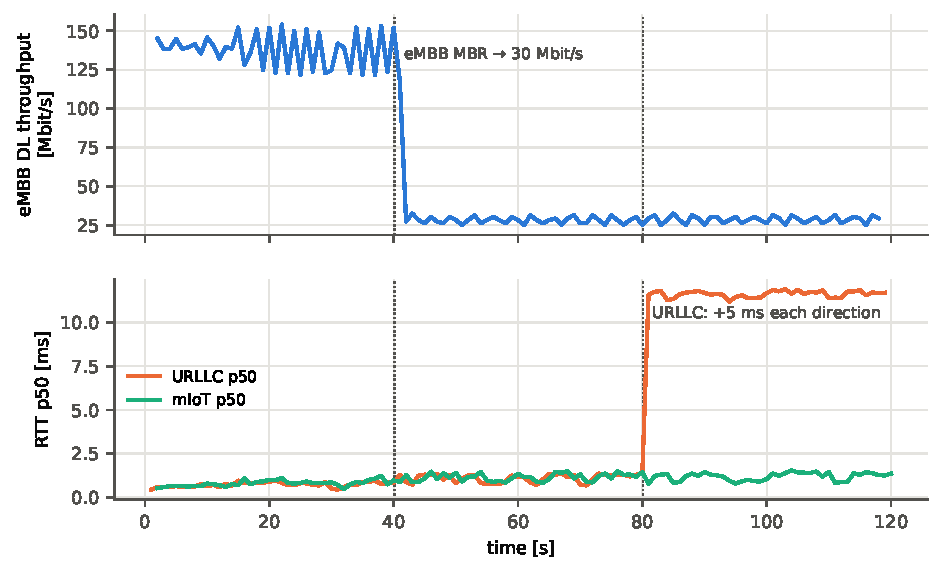
\includegraphics[width=0.78\linewidth]{figures/fig_e4_live.pdf}
\caption{E4: live MBR change on eMBB at $t$\,=\,40\,s and live delay change on URLLC at
$t$\,=\,80\,s (dotted lines, from the event log).}\label{fig:e4}
\end{figure}

\subsection{E5 -- Dedicated vs.\ shared user plane for URLLC}\label{sec:e5}
To test the design decision of \S\ref{sec:slices}, the URLLC probe (200\,Hz) ran under an
identical eMBB overload in two configurations. In \emph{dedicated} mode URLLC is anchored on
UPF-B. In \emph{shared} mode the SMF/UPF-A configs put the \code{urllc} DNN on UPF-A, the
same UPF as eMBB. To make the offered load identical in both modes, eMBB was a fixed-rate UDP
flood (2 UEs $\times$ 500\,Mbit/s downlink) with Session-AMBR and the tc MBR lifted. The
modes were alternated over three repetitions each, so that host drift affects both equally.
During the load phase the VM had no idle CPU. The iperf3 senders alone used about 3 of the 4
vCPUs, followed by \code{open5gs-upfd} (23--42\,\%) and \code{nr-gnb} (20--41\,\%). This is a
deliberately extreme stress test, not an operating point.

\begin{figure}[H]\centering
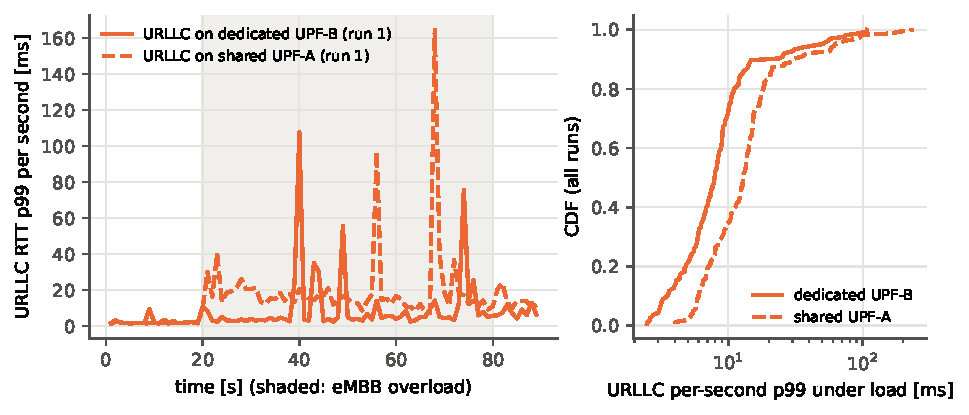
\includegraphics[width=0.86\linewidth]{figures/fig_e5_upf.pdf}
\caption{E5: URLLC per-second p99 RTT in the first run of each mode (left), and the CDF over
all three runs per mode (right, log scale). Shaded: eMBB overload.}\label{fig:e5}
\end{figure}

\begin{table}[H]\centering\small
\caption{E5 summary (mean $\pm$ s.d.\ over 3 runs per mode of the per-run median during load).}\label{tab:e5}
\resizebox{\linewidth}{!}{\begin{tabular}{lrrrrrrr}
\toprule
URLLC user plane & runs & load p50 [ms] & load p99 [ms] & p95 of p99 [ms] & worst p99 [ms] & loss [\%] & eMBB [Mbit/s] \\
\midrule
dedicated & 3 & 1.50 ± 0.86 & 7.42 ± 2.34 & 43.21 ± 9.97 & 107.5 & 11.937 & 58 \\
shared & 3 & 3.77 ± 1.90 & 11.78 ± 4.27 & 59.50 ± 22.36 & 237.4 & 4.831 & 41 \\
\bottomrule
\end{tabular}
}
\end{table}

Sharing the UPF made URLLC latency worse (Fig.~\ref{fig:e5}, Table~\ref{tab:e5}). Pooled over
all load seconds, the median of the per-second p99 rose from 7.9\,ms (dedicated) to 12.9\,ms
(shared). The share of seconds meeting the 10\,ms p99 target fell from 72\,\% to 35\,\%
(Mann--Whitney $p<10^{-11}$; the per-second samples are autocorrelated, so this overstates
the significance). At the correct statistical unit (one value per run, $n$\,=\,3 per mode),
the shared configuration has a 2.5$\times$ higher median RTT and a 1.6$\times$ higher p99, but
Welch's test gives $p$\,=\,0.16 and 0.22. The direction is consistent in two of three
pairs, but more repetitions would be needed to claim significance. URLLC \emph{loss} was
substantial in both modes and, unexpectedly, higher with the dedicated UPF (11.9 vs.\
4.8\,\%). Packets are dropped in components that both modes share, the user-space gNB/UE
(RLS) and the starved CPU, which UPF separation cannot isolate.


\section{Analysis: from scenario to measured result}\label{sec:analysis}
Table~\ref{tab:thread} closes the loop from each scenario requirement (Table~\ref{tab:req})
through the architectural mechanism that serves it to the evidence that it works.

\begin{table}[H]\centering\small
\caption{Traceability: requirement $\rightarrow$ design $\rightarrow$ traffic $\rightarrow$ measured result.}\label{tab:thread}
\begin{tabularx}{\linewidth}{>{\raggedright}p{3.0cm}>{\raggedright}p{3.6cm}>{\raggedright}p{2.5cm}>{\raggedright\arraybackslash}X}
\toprule
Requirement & Mechanism (\S\ref{sec:slices}, \S\ref{sec:arch}) & Traffic & Evidence\\
\midrule
Three services must be logically separated & 3 S-NSSAIs, NSSF/AMF/SMF slice support, per-UE subscription & -- & Allowed/Rejected NSSAI per UE (Tab.~\ref{tab:nssai}); unsubscribed slice refused (E1)\\
Each slice has its own anchor and addressing & DNN$\rightarrow$UPF selection, per-DNN pools and tun & ICMP per session & GTP-U to 10.10.0.1 vs 10.10.0.3 (Lst.~\ref{lst:gtpu}); PFCP 5$\times$UPF-A, 2$\times$UPF-B\\
UE reaches the external DN & N3/N6 namespaces, DN routes, NAT & ping, iperf3, HTTP & 7/7 sessions, 0\,\% loss; 138/18.7/2.1\,Mbit/s; HTTP 200\\
eMBB high rate but capped & HTB MBR + Session-AMBR & on/off TCP & goodput at 92--94\,\% of cap (E1, E3, E4)\\
URLLC p99\,$<$\,10\,ms and lossless under eMBB load & dedicated UPF-B, MBR on eMBB & 100\,Hz probe & p99 0.86\,ms, worst 1.43\,ms, 0\,\% loss while eMBB at cap (E3)\\
mIoT reliable delivery & shared UPF-A, low AMBR & Poisson, 400--1000 devices & 0\,\% loss, ACK p99 $\approx$1--2\,ms (E3)\\
Operator can retune a slice live & tc class/qdisc change via sandbox & all slices & MBR and delay changes take effect within 1\,s, other slices unaffected (E4)\\
Dedicated URLLC user plane worthwhile & UPF-B vs.\ shared UPF-A & UDP overload & median p99 7.9 vs.\ 12.9\,ms; 72\,\% vs.\ 35\,\% of seconds within target (E5)\\
\bottomrule
\end{tabularx}
\end{table}

\paragraph{What the results mean for the scenario.} Within its normal operating envelope
(eMBB at or below its MBR), the factory network meets every requirement of
Table~\ref{tab:req}. The decisive mechanism is the \emph{rate cap on the aggressive slice}.
With eMBB held at its MBR, URLLC and mIoT saw no loss and sub-2\,ms p99 even when eMBB was
saturating (E3). Once that cap is removed and the platform is overloaded (E5), every slice
suffers, because the gNB, the RLS link and the CPU are shared. A dedicated UPF then still
shifts the URLLC latency distribution down, but it does not prevent loss. The practical
lesson is that slice isolation must be enforced at \emph{every} shared resource. In this
testbed those are the transport (tc) and the UPF. In a real network the RAN scheduler is the
most important one, and it is precisely what a software-only RAN cannot model
(\S\ref{sec:limits}).

\paragraph{Signalling cost.} One registration plus one PDU session costs about 12 NGAP
messages, 4 PFCP messages and about 25 distinct SBI requests per UE. The capture holds 82
NGAP frames and 354 non-NRF SBI requests for 7 UEs, the latter seen twice via the SCP. That
amounts to 20--30\,ms of core processing on this platform (Table~\ref{tab:sigtime}). For a
multi-slice UE the PDU procedure runs once per S-NSSAI. Both requests are handled in
parallel: the two PFCP sessions on UPF-A and UPF-B are created within 0.6\,ms of each other
(Fig.~\ref{fig:ladder}). The second N2 response arrives about 200\,ms later only because of
UERANSIM's internal timer.

\paragraph{Reading the latency numbers.} The absolute RTTs (0.3--1.1\,ms median) are the
core and transport cost only; they include no air interface. They are also modulated by the
VM's CPU state (E7): an idle VM looks \emph{slower} than a busy one, so we only compare
measurements taken under like-for-like load. For URLLC dimensioning, the relevant results
are the relative ones: the 10\,ms increase produced by a 5\,ms/direction transport impairment
(E4), and the distribution shift caused by UPF sharing (E5).

\section{Limitations of a software-only environment}\label{sec:limits}
The testbed exercises real 3GPP control-plane procedures and a real GTP-U user plane, so the
\emph{functional} conclusions transfer to a hardware deployment: correct slice selection,
subscription enforcement, per-slice UPF anchoring and the effect of the slice controls. The
\emph{quantitative} conclusions do not transfer directly, for the following reasons.

\begin{enumerate}
\item \textbf{No radio.} RLS replaces the entire NR stack below RRC/NAS. There is no PHY, no
  HARQ, no MAC scheduler, no numerology and no fading or interference. The air-interface
  latency (normally 0.5--4\,ms in the RAN user plane, depending on numerology and
  configured/dynamic grants) and its variability are absent. Slicing \emph{inside} the gNB
  (PRB partitioning, slice-aware scheduling) cannot be studied at all; our slice isolation
  is implemented in the core/transport only. Our sub-millisecond URLLC RTTs are therefore a
  lower bound on the processing cost of the core and transport, not a prediction of
  end-to-end URLLC latency.
\item \textbf{Shared, virtualised CPU.} Every NF, the gNB, all UEs, the traffic generators and
  the DN run on 4 vCPUs of one laptop SoC. Two artefacts follow and are quantified in this
  report. (i) CPU power management: an idle VM gives \emph{higher} RTT than a busy one
  (E7: p50 1.08\,ms idle vs.\ 0.10\,ms with pure busy-loops), so ``latency under load''
  comparisons must use the same CPU state. (ii) Scheduler noise: isolated per-second p99
  spikes of 5--27\,ms appear in every condition, including idle, and are caused by host or
  hypervisor scheduling, not by the 5G stack. We therefore compare medians and distributions
  over repeated runs rather than single worst cases.
\item \textbf{Throughput ceilings are CPU ceilings.} The 300--400\,Mbit/s eMBB maximum reflects
  user-space GTP-U processing in \code{nr-gnb}/\code{nr-ue} and \code{open5gs-upfd}, not any
  radio capacity. Absolute throughput numbers should not be extrapolated.
\item \textbf{Slice QoS enforcement.} Open5GS's UPF polices Session-AMBR (with up to about
  +15\,\% overshoot, \code{results/ambr\_check.txt}), but it does not schedule by 5QI or ARP.
  Differentiation by 5QI is therefore only signalled, not enforced. Our tc layer adds
  per-slice MBR and transport delay/loss, but it is a model of transport impairment, not of
  RAN scheduling.
\item \textbf{Clocks and measurement.} Only RTT is measured, because one-way delay would need
  synchronised clocks across processes. Per-second aggregation hides sub-second dynamics, and
  the 1-s KPI rows mean that the sandbox reacts with up to 2\,s of display lag.
\item \textbf{Scale.} Six UEs and 3000 virtual sensors behind two gateway UEs do not reproduce
  the RACH and signalling load of thousands of real devices. The mIoT result validates only
  the slice's user plane.
\item \textbf{One measured host.} Every number comes from the macOS host. A Windows PC runs
  the same software on a different CPU, hypervisor (Hyper-V) and kernel (Microsoft's WSL
  kernel), so its absolute latencies, throughput ceilings and CPU artefacts will differ. The
  Windows path is supported by the scripts. Its kernel prerequisites are checked by
  \code{wsl\_setup.sh}, which was itself validated in the Linux VM, but the experiments have
  not yet been repeated on a Windows PC.
\end{enumerate}

\noindent\textbf{Validity of conclusions.} The claims that \emph{do} hold:
(a) the end-to-end 5G procedures and slice selection work as specified;
(b) a per-slice control (MBR, delay) is applied within one KPI interval and affects only its
slice;
(c) with eMBB held at its MBR, URLLC and mIoT are unaffected by an eMBB surge;
(d) under platform overload, moving URLLC onto the eMBB UPF shifts its latency distribution
upwards. The per-run effect is consistent in direction but not yet statistically
significant with three runs per mode (\S\ref{sec:e5}).
Claims about absolute latency budgets against TS~22.104 targets would need a hardware or
PHY-emulating RAN (e.g.\ OAI/srsRAN with an SDR, or OAI's RF simulator) and a dedicated core host.

\section{Challenges and resolutions}\label{sec:challenges}
\begin{table}[H]\centering\small
\caption{Problems met during implementation and integration, in the order encountered.}\label{tab:challenges}
\begin{tabularx}{\linewidth}{>{\raggedright}p{4.3cm}>{\raggedright}X>{\raggedright\arraybackslash}p{4.4cm}}
\toprule
Challenge & Root cause & Resolution\\
\midrule
No Linux kernel on the Mac (SCTP, TUN, netns, tc needed) & macOS lacks these features; Docker Desktop is not installed and images are mostly amd64 & Lima VM (Apple Virtualization, arm64 Ubuntu); native arm64 packages, no emulation\\
Homebrew refused to install Lima & Xcode licence not accepted (needs \code{sudo}) & a team member accepted the licence once; documented in the README\\
Provisioning script failed half-way with a syntax error & the script was edited while bash was still executing it (bash reads scripts incrementally) & re-ran the idempotent script; never edit a running script\\
\code{open5gs-dbctl} not found & not shipped in the Ubuntu \code{.deb} & fetched from the matching v2.8.0 tag in \code{00\_provision.sh}\\
\code{update\_slice} created sessions without QoS/AMBR & helper only writes the DNN & \code{mongosh} pass sets 5QI/ARP/AMBR for every session by DNN\\
GBR 5QI~82 risky for URLLC default flow & GBR needs GBR/MBR values and PCC rules & switched to non-GBR low-latency 5QI~80\\
Downlink could bypass the UPF & UE and core on the same host: replies to a local UE address are delivered locally & UEs/gNB moved into netns \code{ran}; verified with GTP-U in the capture\\
URLLC RTT appeared to be 20\,ms & probe only read echoes on its 10\,ms send tick & \code{select()} until the next deadline; RTT timestamped on arrival\\
``Slice down'' did not stay down & UERANSIM re-establishes configured sessions $\approx$200\,ms after release & admin state + switch-off deregistration + re-attach with filtered config\\
No NAS details in Wireshark after Security Mode & integrity-protected NAS with NEA0 is not shown by default & \code{nas-5gs.null\_decipher:TRUE}; AMF ciphering order NEA0 first\\
\code{tshark} display filter rejected & Wireshark 4.2 needs commas in set syntax & \code{pfcp.msg\_type in \{50,51,52,53\}}\\
DNS failed inside UE namespace & \code{ran} netns cannot reach the VM's stub resolver & resolve in the core netns, pass \code{curl --resolve}\\
eMBB throughput spikes in plots & iperf3's trailing partial interval and duplicate samples per second & drop intervals $<$0.5\,s; average per UE before summing\\
URLLC faster under load than idle & VM CPU idle-state wake-up latency & control experiment E7; compare only like-for-like CPU states\\
First E5 run inconclusive & TCP eMBB load varied 270--1600\,Mbit/s between runs (AMBR, TCP dynamics), confounding the comparison & fixed-rate UDP load, AMBR lifted, 3 alternating repetitions per mode\\
Stale UE routes after restarts & UERANSIM leaves its \code{ip rule} entries in netns \code{ran} & \code{stop\_ran.sh} flushes them\\
\bottomrule
\end{tabularx}
\end{table}

\section{Conclusions and future work}\label{sec:conclusion}
We built a complete, reproducible 5G SA system with three differentiated slices on a single
laptop, using only open-source software. Open5GS and UERANSIM ran natively on arm64 inside a
Lima VM on macOS, and the same scripts also target Windows through WSL2. Namespaces enforced
a realistic RAN/core/DN separation. The scenario,
architecture, traffic and measurements form one thread. The factory's three service classes
became three S-NSSAIs with their own DNN, pool, QoS profile and, for URLLC, their own UPF. The
signalling shows each UE receiving exactly its subscribed Allowed NSSAI and each PDU session
being anchored on the intended UPF. The KPIs show that the slice controls work and are
isolated. Capping the eMBB slice was enough to keep URLLC lossless with a p99 below 1.5\,ms during an
eMBB surge. Under deliberate platform overload, a dedicated URLLC UPF cut the share of
seconds that missed the 10\,ms p99 target from 65\,\% to 28\,\%, but it could not prevent losses in the shared RAN
components.
The sandbox exposes all of this to a non-expert in one page.

\paragraph{Future work.}
(1) Replace RLS with a PHY-level RAN (OpenAirInterface or srsRAN Project with its RF
simulator or an SDR) to study slice-aware MAC scheduling.
(2) Add an O-RAN near-RT RIC (FlexRIC or O-RAN SC) with an xApp that retunes slice resources
from the KPIs the sandbox already collects, closing the loop automatically.
(3) Enforce QoS by 5QI with PCC rules and GBR flows for URLLC.
(4) Move the NFs to Kubernetes/Helm with CPU pinning, so that the CPU artefacts of
\S\ref{sec:limits} can be controlled.
(5) Scale mIoT with a UE simulator that supports thousands of real registrations.

\clearpage
\bibliographystyle{unsrt}
\bibliography{refs}
\end{document}
